\chapter{Entwurf / Design}



\section{Architekturentscheidung}

\textbf{Kontextsicht}\newline
Zeigt die Zusammenh�nge zwischen dem System und seinen Nachbarsystemen.\newline
\textbf{Bausteinsicht}\newline
Zeigt die statische Struktur, welche Bausteine Teil der Anwendung sind und welche
Beziehung sie zueinander haben.\newline
\textbf{Laufzeitsicht}\newline
Zeigt die Abl�ufe der Anwendung und die Zusammenarbeit der Bausteine zur Laufzeit.\newline
\textbf{Verteilungssicht}\newline
Zeigt, in welcher Umgebung das System abl�uft.

\section{Kontextabgrenzung}
Dieser Abschnitt stellt das Umfeld von der Applikation dar. Fu?r welche Benutzer ist es da, und mit welchen Fremdsystemen interagiert es?

\begin{center}
 \begin{minipage}{\linewidth}
	\centering
	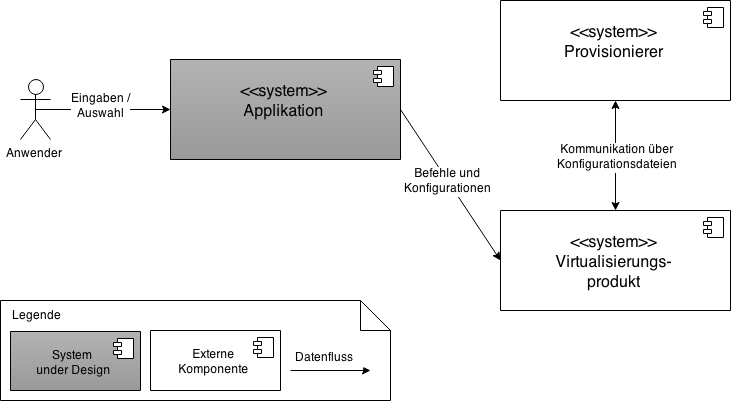
\includegraphics[scale=0.5]{../Bilder/kontextsicht.png}
	\captionof{figure}[kurze Bildunterschrift]{Bildunterschrift}
 \end{minipage}
\end{center}

In der dargestellten Kontextsicht, wird die d
\chapter{Sichten}
\section{Bausteinsicht}
\section{Laufzeitsicht}
\section{Verteilungssicht}
\section{Zusammenfassung}
